Uma solução saturada de nitrato de potássio (\chemfig{KNO_3}) constituída, além do sal, por $100$ g de água, está à temperatura de $70$ $^\circ$C.
Essa solução é resfriada a $40$ $^\circ$C, ocorrendo precipitação de parte do sal dissolvido.
Com base nesses dados e no gráfico apresentado abaixo:

Gráfico da solubilidade do nitrato de potássio em função da temperatura.

\begin{center}

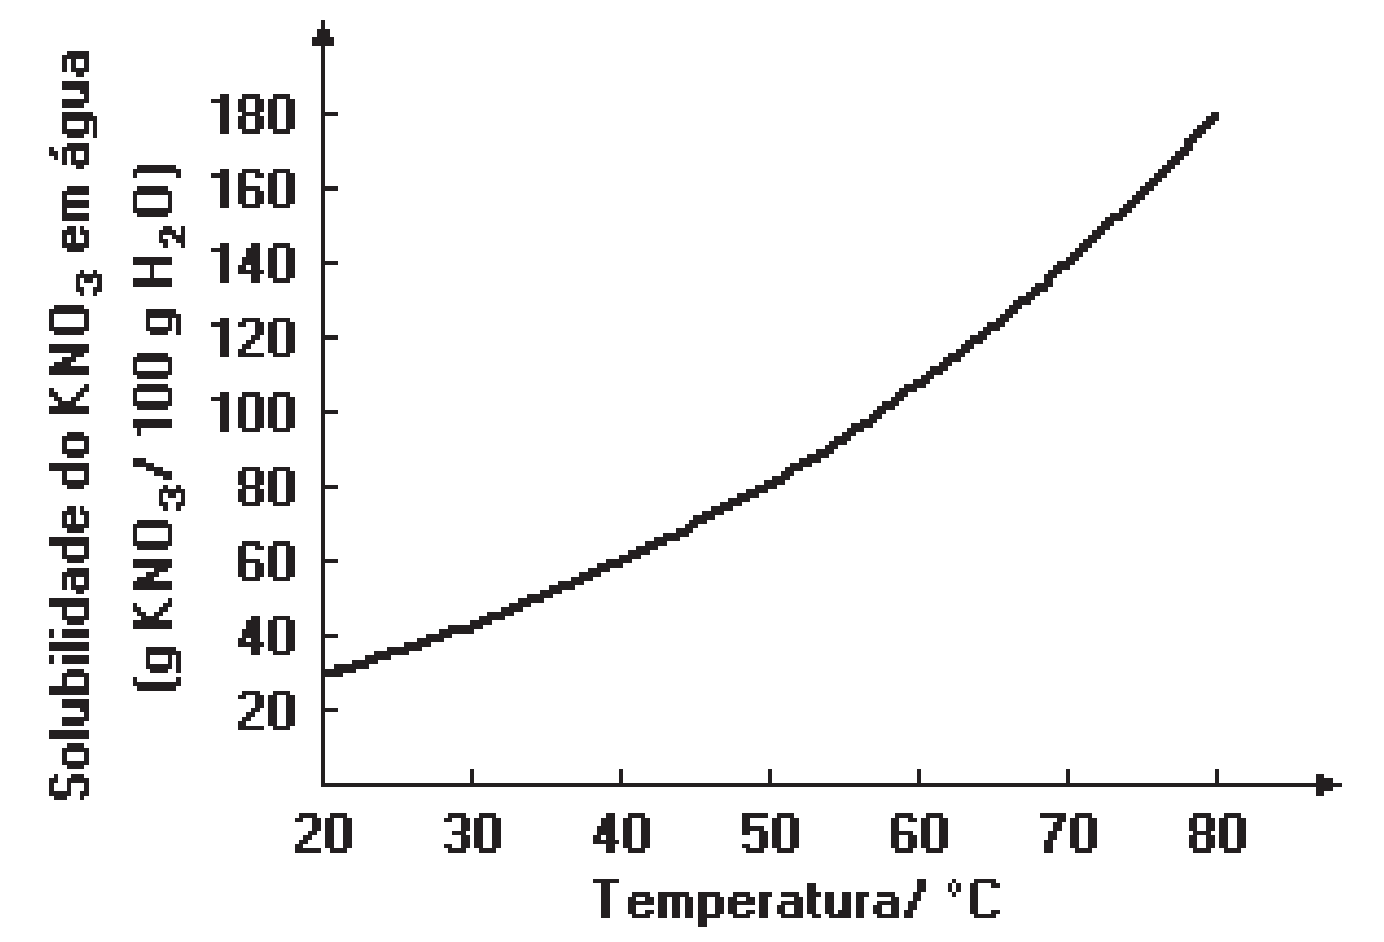
\includegraphics[width = 7cm]{figure.png}

\end{center}

Pode-se afirmar que a massa de sal que precipitou foi de aproximadamente:

\begin{enumerate}[label = (\alph*)]
	\item $20$ g
	\item $40$ g
	\item $60$ g
	\item $80$ g
	\item $100$ g
\end{enumerate}
